\section{Expressive Power}\label{expressivity}

In this section we compare the expressive power of memory logics
with respect to both the modal and hybrid logics.
But comparing the expressive power of these logics poses a complication
because, strictly speaking, each of them uses a different class of models.
We would like to be able to define a natural mapping between models
of each logic, similar to the natural mapping that exists between
Kripke models and first-order models~\cite{BRV01}.

Such a mapping is easy to define in the case of $\cMLRKE$ where the model is interpreted with $S=\emptyset$: each
Kripke model $\diam{W,\rels,V}$ can be identified with the $\cMLRKE$
model $\diam{W,\rels, V, \emptyset}$. Similarly, for formulas
which are sentences, the $\cMLRKE$ model $\diam{W,\rels,V,\emptyset}$ can be identified with the hybrid model
$\diam{W,\rels,V,g}$ (for $g$ arbitrary).
%
Since models for the $\cMLRKE$ logic coincide with those of
$\cMLRKME$, the same applies for the mapping between Kripke models
and $\cMLRKME$ models.
%
As we will discuss below, it is harder to find such a natural way to
transform models for the case of $\cMLRK$ and $\cMLRKM$: the most
natural way seems to involve a shift in the signature of the
language.

\begin{defn}[$\mathcal{L} \le \mathcal{L'}$]
We say that
$\mathcal{L'}$ is \emph{at least as expressive as} $\mathcal{L}$
(notation $\mathcal{L} \le \mathcal{L'}$) if it is possible to
define a function $\Tr$ between formulas of  $\mathcal{L}$ and $\mathcal{L'}$
such that for every model $\model$ and every formula $\varphi$ of $\mathcal{L}$
we have that
\[
\model \models_\mathcal{L} \varphi \mbox{ iff } \model \models_{\mathcal{L}'} \Tr(\varphi).
\]

We say that $\mathcal{L'}$ is \emph{strictly more expressive} than $\mathcal{L}$
(notation $\mathcal{L} < \mathcal{L'}$) if $\mathcal{L} \le \mathcal{L'}$ but
not $\mathcal{L}' \le \mathcal{L}$.  And we say that $\gL$ and $\gL'$ are equally
expressive (notation $\gL = \gL'$) if $\gL \le \gL'$ and $\gL' \le \gL$.
\end{defn}

\begin{figure}
\begin{center}
\begin{tikzpicture}[>=latex]
  \node[draw,rounded corners,minimum height=2.5cm,minimum width=1cm] (b1) at (3,1.25) {};
  \node[draw,rounded corners,minimum height=2.5cm,minimum width=1cm] (b2) at (5,1.25) {};
    \node[draw,rounded corners,minimum height=2.5cm,minimum width=1.4cm] (b3) at (7,1.25) {};

  \node (n0) at (1.2,1.25) {$\mathcal{K}$};
  \node (n3) at (3,2) {$\cMLRKM$};%L3
  \node (n4) at (3,.5) {$\cMLRKME$};%L4
  \node (n1) at (5,2) {$\cMLRK$};%L1
  \node (n2) at (5,.5) {$\cMLRKE$};%L2
  \node (n5) at (7,2) {$\cMLS$};%L5
  \node (n6) at (7,.5) {$\hlogic$};%HL

  \draw [->] (n0) -- (b1);
  \draw [->] (b1) -- (b2);
  \draw [->] (b2) -- (b3);

  \draw [<->,dashed] (n3) edge (n4);
  \draw [<->,dashed] (n1) edge (n2);
  \draw [<->] (n5) edge (n6);
\end{tikzpicture}
\end{center}
\caption{Expressive power hierarchy.}\label{fig-expressivity}
\end{figure}


The summary of the results we are going to establish in this section
is shown in Figure~\ref{fig-expressivity}.  In the figure, a full arrow
between two logics $\gL$ and $\gL'$ means that $\gL < \gL'$. Double headed
arrows link languages with the same expressive power.  We use dashed
arrows when a change in the signature is required in the proof, and this is
the first result we are going to show.

\tb{SS: no hay double headed arrows. Entre $\hlogic$ y stack hay
cambio de signatura? Si no hay, deberia ser double headed arrow}

\begin{thm} \
\begin{enumerate}
\item $\cMLRKE$ over the signature $\diam{\prop \cup \{\mathit{known}\}, \rel}$ is equivalent to $\cMLRK$ over the signature $\diam{\prop, \rel}$
\item $\cMLRKME$ over the signature $\diam{\prop \cup \{\mathit{known}\}, \rel}$ is equivalent to $\cMLRKM$ over the signature $\diam{\prop, \rel}$
\end{enumerate}
\end{thm}

\begin{pf}
The argument for item $2$ is exactly the same as the one for item $1$.  Hence let's
prove $\cMLRKE=\cMLRK$ (over the appropriate signatures).

We start by associating every model $\gM=\tup{W,\rels,V,S}$ of $\cMLRK$ over the signature $\diam{\prop, \rel}$ with the model $\gM'=\tup{W,\rels,V',\emptyset}$
of $\cMLRKE$ over the signature $\diam{\prop \cup \{\mathit{known}\}, \rel}$ where $V'$ is identical to $V$ over $\prop$ and $V'(\mathit{known}) =S$.
\smallskip

\noindent $[\cMLRKE \le \cMLRK]$: use the translation $\Tr$ that
only rewrites the propositional symbol $\mathit{known}$ as $\known$
in any formula of $\cMLRKE$. Clearly for any formula $\varphi \in
\cMLRKE$ we have that $\gM',w \models \varphi$ iff $\gM,w \models
\Tr(\varphi)$.
\smallskip

\noindent $[\cMLRK \le \cMLRKE]$: use the translation $\Tr$ that
only rewrites $\known$ as $(\known \vee \mathit{known})$ in any
formula of $\cMLRK$. Clearly for any formula $\varphi \in \cMLRK$ we
have that $\gM,w \models \varphi$  iff $\gM',w \models
\Tr(\varphi)$.
\end{pf}

On the other hand, the freedom to decide when to remember one state
gives $\cMLRK$ and $\cMLRKE$ more expressive power when compared
with $\cMLRKM$ and $\cMLRKME$.


\begin{thm}\label{thm:four-le-two}
$\cMLRKM < \cMLRK$ and $\cMLRKME < \cMLRKE$.
\end{thm}

\begin{pf}
We only prove the result for $\cMLRKM < \cMLRK$ as the other case is
identical.
\smallskip

\noindent
$[\cMLRKM \leq \cMLRK]$: It is easy to see that there is a translation \Tr\ from $\cMLRKM$-
to $\cMLRK$-formulas which maps $\ttup{r}\varphi$ to
$\remember\diam{r}\varphi$ and verifies $\model \models_{\cMLRKM}
\varphi$ iff $\model \models_{\cMLRK} \Tr(\varphi)$.
\smallskip

\noindent
$[\cMLRK \not\leq \cMLRKM]$: Let
$\model_1=\diam{\{w,v,r\}, R_1, V_1, \emptyset}$ and
$\model_2=\diam{\{w,v,r\}, R_2, V_2, \emptyset}$ such that
$R_1=\{(w,v),(v,r),(r,w)\}$, $R_2=\{(w,v),(v,r),(r,v)\}$ and $V_1(p)
= V_2(p) = \emptyset$ for all $p \in \prop$, as shown below:
%in Figure~\ref{fig:L3L1}.
%\begin{figure}
\begin{center}
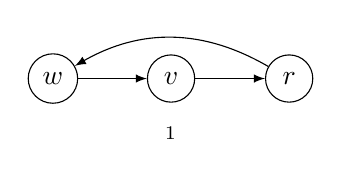
\begin{tikzpicture}[>=latex]
  \node (n1) at (0,0) [shape=circle,draw,minimum height=.6cm] {$w$} ;
  \node (n2) at (1.5,0) [shape=circle,draw,minimum height=.6cm] {$v$} ;
  \node (n3) at (3,0) [shape=circle,draw,minimum height=.6cm] {$r$} ;

  \draw [->] (n1) -- (n2);
  \draw [->] (n2) -- (n3);
  \draw [->] (n3) edge[bend right=30] (n1);

  \node at (1.5,-.7) {$\model_1$};
\end{tikzpicture}
\hspace{1cm}
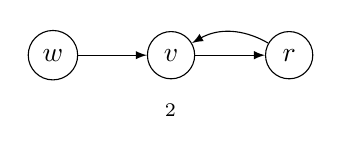
\begin{tikzpicture}[>=latex]
  \node (n1) at (0,0) [shape=circle,draw,minimum height=.6cm] {$w$} ;
  \node (n2) at (1.5,0) [shape=circle,draw,minimum height=.6cm] {$v$} ;
  \node (n3) at (3,0) [shape=circle,draw,minimum height=.6cm] {$r$} ;

  \draw [->] (n1) -- (n2);
  \draw [->] (n2) -- (n3);
  \draw [->] (n3) edge[bend right=30] (n2);

  \node at (1.5,-.7) {$\model_2$};
\end{tikzpicture}
\end{center}
%\caption{$\cMLRKE\not=\cMLRKME$.}
%\label{fig:L3L1}
%\end{figure}

We prove that $\model_1$ and $\model_2$ are $\cMLRKM$-bisimilar. As
every state in both models has a unique successor, Duplicator has
only one way of playing, and this only way is indeed a winning
strategy. From this follows that no formula in $\cMLRKM$ can
distinguish $\model_1$ and $\model_2$. On the other hand, let
$\varphi = \diam{r}\remember\diam{r}\diam{r}\known$ be a
$\cMLRK$-formula. It is easy to see that $\model_1,w \not \models
\varphi$, but $\model_2, w \models \varphi$.
\end{pf}


We will now compare the expressive power of memory logics with
the basic modal logic $\bml$.

\subsection{Memory Logics and Modal Logics}

Because models of $\K$ are different from models for memory logics
we should start by defining how are we going to match them.  In this
case, it seems that we don't have other option but to change the
signature.  But even over a suitable extended signature, $\bml$ is
less expressive than $\cMLRKM$.
It is not difficult to see intuitively that $\remember$ and $\known$ do bring
additional expressive power into the language of $\bml$: with their
help we can detect cycles in a given model, while formulas of $\K$
are invariant under unraveling.

\begin{thm}\label{teo:bml_ml}
$\bml$ over the signature $\diam{\prop \cup \{known\}, \rel}$ is
strictly less expressive than both $\cMLRKM$ and $\cMLRKME$ over the signature
$\diam{\prop, \rel}$.
\end{thm}

\begin{pf}
We only prove the result for $\bml$ and $\cMLRKM$, the other case is identical. Showing that $\bml\leq\cMLRKM$ is straightforward as $\bml$ is a
sub-language of $\cMLRKM$.  Hence, we can take $\Tr$ to be the
identity function.

To see that $\cMLRKM\not\leq\bml$, let
$\model_1=\diam{\{w\},\{(w,w)\},V_1}$ and
$\model_2=\langle \{u,v\}, \{(u,v)$, $(v,u)\},V_2\rangle$, where
$V_1(p) = V_2(p) = \emptyset$ for all $p \in \prop \cup \{known\}$
 be two Kripke models as shown below:
%in Figure~\ref{fig:L3K}.
\begin{center}
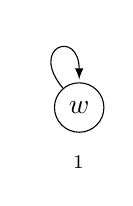
\begin{tikzpicture}[>=latex]
  \node (n1) at (0,0) [shape=circle,draw,minimum height=.6cm] {$w$} edge [in=90, out=130,loop] ();

  \node at (0,-.7) {$\model_1$};
\end{tikzpicture}
\hspace{2cm}
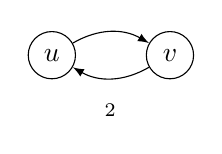
\begin{tikzpicture}[>=latex]
  \node (n2) at (0,0) [shape=circle,draw,minimum height=.6cm] {$u$} ;
  \node (n3) at (1.5,0) [shape=circle,draw,minimum height=.6cm] {$v$} ;

  \draw [->] (n2) edge[bend left=30] (n3);
  \draw [->] (n3) edge[bend left=30] (n2);

  \node at (.75,-.7) {$\model_2$};
\end{tikzpicture}
\end{center}

It is known that the models are $\bml$ bisimilar
(see~\cite{BRV01}). On the other hand, they can be distinguished
by the $\cMLRKM$-formula $\remember \ttup{r}\known$.
%
%\begin{figure}
%\caption{$\cMLRKM\not=\bml$.}
%\label{fig:L3K}
%\end{figure}
%
\end{pf}

\tb{C: we won't say anyting about $\cMLRKME$ is that ok? \\SS: agregamos ese resultado en el teo de arriba, a eso te referias? Del lado de K vs memory logics es la flecha que faltaba mencionar}


\subsection{Memory Logics and Hybrid Logics}

We will now compare the expressive power of memory logics with
respect to hybrid logics.  The most natural choice for the
comparison is the hybrid logics $\hlogic$.
We will prove that $\hlogic$ is strictly more expressive than $\cMLRKE$.
Intuitively,
$\downarrow$ can easily simulate $\remember$, but $\known$ does not
distinguish between different memorized states (while nominals
bound by $\downarrow$ do distinguish them).



\begin{thm}\label{thm:tle_leq_hlogic}
$\cMLRKE < \hlogic$.
\end{thm}

\begin{pf}
We first prove that $\cMLRKE \le \hlogic$. We define
the translation $\Tr$, taking $\cMLRKE$-formulas over the signature
$\diam{\prop,$ $\rel}$ to $\hlogic$ sentences over the signature
$\diam{\prop, \rel, \nom}$. $\Tr$ is defined for any finite set $N
\subseteq \nom$ as follows:
$$
\begin{array}{rcl}
\Tr_N(p) & = & p \quad p \in \prop\\
\Tr_N(\known) & = & \bigvee_{i \in N} i \\
\Tr_N(\lnot \varphi) & = & \lnot \Tr_N(\varphi) \\
\Tr_N(\varphi_1 \land \varphi_2) & = & \Tr_N(\varphi_1) \land \Tr_N(\varphi_2) \\
\Tr_N(\diam{r} \varphi) & = & \diam{r} \Tr_N(\varphi) \\
\Tr_N(\remember \varphi) & = & \down i. \Tr_{N\cup\{i\}}(\varphi)
\quad \textrm{where $i \notin N$.}
\end{array}
$$

\noindent A simple induction shows that $\model, w \models \varphi$
iff $\model, g, w \models \Tr_\emptyset(\varphi)$, for any $g$.
\smallskip


Now we prove that $\hlogic$ is strictly more expressive than $\cMLRKE$.
Let $\model_1=\diam{\omega,R_1,\emptyset,\emptyset}$ and
$\model_2=\diam{\omega,R_2,\emptyset,\emptyset}$, where $R_1=\{(n,m)
\mid n\not= m\} \cup \{(0,0)\}$ and $R_2=\{(n,m) \mid n\not= m\}
\cup \{(0,0),(1,1)\}$. Graphically,

\begin{center}
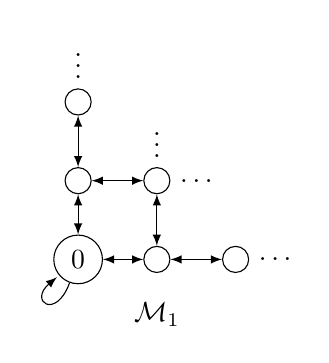
\begin{tikzpicture}[>=latex]

  \node (n11) at (0,0) [shape=circle,draw] {0} edge [in=220, out=250,loop] ();
  \node (n22) at (1,1) [shape=circle,draw, label=right:$\dots$, label=above:$\vdots$] {};
  \node (n12) at (0,1) [shape=circle,draw] {} ;
  \node (n21) at (1,0) [shape=circle,draw] {};
  \node (n13) at (0,2) [shape=circle,draw, label=above:$\vdots$] {};
  \node (n31) at (2,0) [shape=circle,draw, label=right:$\dots$] {};

  \draw [<->] (n11) -- (n12);
  \draw [<->] (n21) -- (n22);
  \draw [<->] (n12) -- (n22);
  \draw [<->] (n11) -- (n21);
  \draw [<->] (n21) -- (n31);
  \draw [<->] (n12) -- (n13);

  \node at (1,-.7) {$\mathcal{M}_1$};

\end{tikzpicture}
\hspace{10mm}
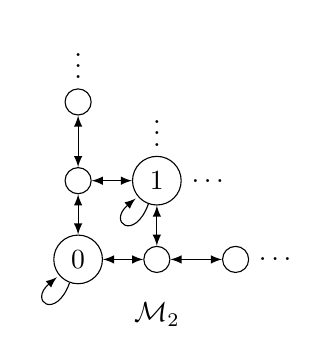
\begin{tikzpicture}[>=latex]

  \node (n11) at (0,0) [shape=circle,draw] {0}
                       edge [in=220, out=250,loop] ();
  \node (n22) at (1,1) [shape=circle,draw, label=right:$\dots$, label=above:$\vdots$] {1}
                       edge [in=220, out=250,loop] ();
  \node (n12) at (0,1) [shape=circle,draw] { } ;
  \node (n21) at (1,0) [shape=circle,draw] { };
  \node (n13) at (0,2) [shape=circle,draw, label=above:$\vdots$] { };
  \node (n31) at (2,0) [shape=circle,draw, label=right:$\dots$] { };

  \draw [<->] (n11) -- (n12);
  \draw [<->] (n21) -- (n22);
  \draw [<->] (n12) -- (n22);
  \draw [<->] (n11) -- (n21);
  \draw [<->] (n21) -- (n31);
  \draw [<->] (n12) -- (n13);

  \node at (1,-.7) {$\mathcal{M}_2$};
\end{tikzpicture}
\end{center}

\noindent where the accessibility relation is the
transitive closure of the arrows shown but without reflexive
loops excepts those explicitly marked.


We prove that $\tup{\model_1,0}\equiv^{\EF} \tup{\model_2,0}$ showing a winning
strategy for Duplicator. Intuitively, the strategy for Duplicator
is as follows: whenever one player is in
$\tup{\model_1,0}$ the other will be in $\tup{\model_2,0}$ or
$\tup{\model_2,1}$, and conversely whenever a player is in
$\tup{\model_1,n}$, $n>0$ the other will be in $\tup{\model_2,m}$, $m>1$.
This is maintained until Spoiler (if ever) decides to remember a
state. Once this is done, then any move leads to a win of Duplicator.

Formally, the winning strategy will have two stages:
\smallskip

\noindent
a) While Spoiler does not remember any reflexive
state, Duplicator plays as follows: if Spoiler
chooses $0$ in any model, Duplicator chooses $0$ in the other;
if Spoiler chooses $n>0$ in $\model_1$, Duplicator plays $n+1$ in
$\model_2$; if Spoiler chooses $n>0$ in $\model_2$, Duplicator plays
$n-1$ in $\model_1$. Notice that with this strategy Spoiler chooses
a reflexive state if and only if Duplicator answers with a reflexive
one. This is clearly a winning strategy.
\smallskip

\noindent
b) If ever Spoiler decides to
remember a reflexive state, Duplicator starts using the following
strategy: if Spoiler selects a state $n$, Duplicator answers with an
agreeing state $m$ of the opposite model. Notice that this is always
possible since both $n$ and $m$ see infinitely many non remembered
states and at least one remembered state.
\smallskip

\noindent
On the other hand, let $\varphi$ be the formula $\down i. \diam{r}(i
\land \diam{r}(\lnot i \land \down i.\diam{r}i))$. It is easy to see
that $\model_1, 0 \not \models \varphi$ but $\model_2, 0 \models
\varphi$.
\end{pf}

\tb{Dieguis cambia la demo de abajo.}

We have shown that $\cMLRKE < \hlogic$ but the proof seems to intrinsically
use infinite models.  Actually, $\cMLRKE < \hlogic$ even on finite models. For this purpose we will first introduce a bounded round version of the EF game:
%
\begin{defn}
We will define the \emph{$n$-round Ehrenfeucht-Fra\"iss\'e game} for a given logic $\mathcal{L}$ $\EF^n(\model_1, \model_2, w_1, w_2)$ as the game in which Spoiler has only $n$ rounds of the game to beat Duplicator. In the case Duplicator has a strategy to remain undefeated for $n$ rounds, he wins the game and we will write $\tup{\gM_1,w_1}\equiv^{\EF}_n\tup{\gM_2,w_2}$.
\end{defn}
%
We will state without a proof the following theorem we will use, that can actually be extended to any of the logics $\mathcal{L}_i$.
\begin{thm}
For any pair of pointed models, $\tup{\gM_1,w_1}\equiv^{\EF}_n\tup{\gM_2,w_2}$ in $\cMLRKE$ if and only if for every formula $\varphi$ of $\cMLRKE$ with modal depth $n$, $\gM_1,w_1\models\varphi$ iff $\gM_2,w_2\models\varphi$.
\end{thm}
%
We can now prove the expected theorem.
\begin{thm}\label{thm:tle_leq_hlogic_fin}
$\cMLRKE < \hlogic$ over the class of finite models.
\end{thm}
\begin{pf}
We will prove that there is an $\hlogic$-expressible property $\varphi$ that cannot be expressed in $\cMLRKE$ over finite models. To do this, for every $n$ we will exhibit two finite models $\gM_1^n,\gM_2^n$ such that $\gM_1^n,w_0\models\varphi$, $\gM_1^n,w_0\not\models\varphi$ but $\tup{\gM_1^n,w_0}\equiv^{\EF}_n\tup{\gM_1^n,w_0}$. This implies that there is no formula of $\cMLRKE$ capable of expressing this property. If there was one $\psi$ with modal depth $m$, then as $\tup{\gM_1^n,w_0}\equiv^{\EF}_m\tup{\gM_2^n,w_0}$,  $\psi$ would be satisfied in either none or both of these models, which is absurd.

Let
\[
 \varphi =
\down i. \diam{R}(i \land \diam{R}(\lnot i \land \down i.
\diam{R}i)),
\]
and let, for $n\geq 1$, $\model^1_n = \diam{W_n, R_1, \emptyset,
\emptyset}$ and $\model^2_n = \diam{W_n, R_2, \emptyset, \emptyset}$
where
\begin{eqnarray*}
W_n&=&\{w_0, \dots, w_{n+1}\}\\
R_1&=&\{(n,m)\mid n \neq m\} \cup \{(w_0,w_0)\}\\
R_2&=&R_1 \cup \{(w_1, w_1)\}.
\end{eqnarray*}
%
Clearly, for every $n \geq 1$, $\model^1_n, w_0 \not\models \varphi$ and
$\model^2_n, w_0 \models \varphi$.

To prove that $\tup{\gM_1^n,w_0}\equiv^{\EF}_n\tup{\gM_2^n,w_0}$, we will describe Duplicator's strategy dividing it again in two stages:
\smallskip

\noindent
a) While Spoiler does not remember any reflexive state,
Duplicator plays with the following strategy: if Spoiler chooses
$w_0$ in any model, Duplicator chooses $w_0$ in the other one; if
Spoiler chooses $w_k$, $0 < k < n+1$, in $\model_1$, Duplicator
plays $w_{k+1}$ in $\model_2$, and if Spoiler chooses $w_{n+1}$ in
$\model_1$, Duplicator plays $w_2$ in $\model_2$; if Spoiler chooses
$w_k$, $k > 0$, in $\model_2$, Duplicator plays $w_{k-1}$ in
$\model_1$. Note that with this strategy, Spoiler chooses a
reflexive state iff Duplicator answers with a reflexive one.

\noindent
b) If ever
Spoiler decides to remember a reflexive state, then from that point
of the game, for every state $w_i$ chosen by Spoiler, Duplicator
will always have an agreeing state $w_j$ on the opposite model he
can choose from. This happens because the models have $n+1$ states, and
therefore there is always at least two non-remembered states. At each round the number of unremembered states can only be decremented by one, and then up to round $n$ both players will always see remembered and unremembered states both from $w_i$ and $w_j$.
\end{pf}

The $\hlogic$-sentence we use in the proofs of Theorem~\ref{thm:tle_leq_hlogic}
and~\ref{thm:tle_leq_hlogic_fin} has only one nominal.
  Hence, we have actually proved that
$\hlogicone\not\le\cMLRKE$, where $\hlogicone$ is $\hlogic$
restricted to only one nominal.  But actually, it is also the case
that $\cMLRKE \not\le\hlogicone$.  More generally, for any fixed
number $k$ of nominals, the logics $\hlogick$ and $\cMLRKE$ are
incomparable.

\begin{thm}
For any fixed $k$, the logics $\hlogick$ and $\cMLRKE$ are incomparable in terms of expressive power.
\end{thm}
\begin{pf}
We will show the proof for $k=1$, the general case being similar.
$\hlogicone\not\leq\cMLRKE$ is a direct consequence of the
proof of Theorem~\ref{thm:tle_leq_hlogic}.

To prove $\cMLRKE \not
\le \hlogicone$, let $\model_1=\diam{\{1,2,3\},\{(i,j) \mid 1 \leq
i,j \leq 3\},V_1,\emptyset}$  and
$\model_2=\diam{\{1,2\},\{(i,j) \mid 1 \leq i,j \leq
2\},V_2,\emptyset}$
where
$V_1(p) = V_2(p) = \emptyset$ for all $p \in \prop$
(a clique of size 3 and 2 respectively). It is easy to check
that $\model_1,1$ and $\model_2,1$ are $\bisim_{\hlogicone}$-bisimilar. However, the
formula
$\varphi = \remember \diam{r} (\neg \known \land \remember
\diam{r} (\neg\known \land \remember \diam{r} \neg\known))$
distinguishes the models: $\model_1,1 \models \varphi$ but
$\model_2,1 \not\models \varphi$.

This result can be extended to $\hlogick$ for any fixed $k$, by taking cliques of the appropriate size.
\end{pf}

\tb{C: I propose We don't say anything about $\cMLRK$ is that ok? Result
commented out below\\
SS: Mirando el grafico de expresividad solo falta demostrar la flecha $L1 < HL(\down)$. Eso creo que deberíamos ponerlo, al menos como un teo sin demostracion, es bastante facil de ver. Con eso se completaria el diagrama. Ahora es el 2do item de lo que esta comentado aca abajo, pero yo creo que lo pondria apenas empieza la subseccion ``Memory Logics and Hybrid Logics'', antes de la demoledora.}


% \begin{thm}\label{thm:expr_power}
% The following results concerning expressive power can be established
% \begin{enumerate}
% \item $\bml$ over the signature $\diam{\prop \cup \{\mathit{known}\}, \rel}$ is strictly
% less expressive than {\em $\cMLRK$} over the signature $\diam{\prop, \rel}$.
% \item {\em $\cMLRK$} over the signature $\diam{\prop, \rel}$ is strictly less expressive
% than $\hlogic$ over the signature $\diam{\prop \cup \{\mathit{known}\}, \rel,\nom}$.
% \end{enumerate}
% \end{thm}
%
% \begin{pf}
% All proofs are similar to (and sometimes easier than) the ones
% presented above. We only discuss 2. To prove $\cMLRK \le \hlogic$ (over
% the appropriate signatures) we adapt the translation $\Tr$ with the
% following clause for $\known$
% $$
% \begin{array}{rcl}
% \Tr_N(\known) & = & \big (\bigvee_{i \in N} i \big) \vee
% \mathit{known}.
% \end{array}
% $$
% $\hlogic \not \le \cMLRK$ can be shown using the following models. Let
% $\model_1=\diam{\{w\},$ $\{(w,w)\},\emptyset,\{w\}}$ and
% $\model_2=\diam{\{u,v\},\{(u,v),(v,u)\},\emptyset,\{u,v\}}$.
% Duplicator always wins on $E(\model_1,\model_2,w,u)$ and thus
% $\model_1,w\bisim_{\cMLRK}\model_2,u$. On the other hand,
% $\model'_1,w\models_{\hlogic}\down i.\diam{r}i$ but
% $\model'_2,u\not\models_{\hlogic}\down i.\diam{r}i$, for $\model'_1,
% \model'_2$ the  models corresponding to $\model_1$ and $\model_2$.
% \end{pf}

To finish this section, we will compare $\cMLS$ with $\hlogic$ and
prove that they are equivalently expressive.  This might come as a
surprise, as we could think that the restricted access to the elements
in the stack might actually limit the expressive power of $\cMLS$.
The proof below shows that it is the possibility to `make copies of
the stack' while evaluating a formula what solves the problem.

\begin{thm}\label{prop:stack_leq_hl}
$\cMLS = \hlogic$.
\end{thm}

\begin{pf}
To prove $\cMLS \le \hlogic$, we define
the translation mapping an $\cMLS$-formula and a list of
nominals $N$ into an $\hlogic$-formula.
\begin{eqnarray*}
\Tr_N(p) & = & p \quad p \in \prop\\
\Tr_N(\lnot \varphi) & = & \lnot \Tr_N(\varphi) \\
\Tr_N(\diam{r} \varphi) & = & \diam{r} \Tr_N(\varphi) \\
\Tr_N(\varphi_1 \land \varphi_2) & = & \Tr_N(\varphi_1) \land \Tr_N(\varphi_2)\\
\Tr_N(\push \varphi) & = & \down i. \Tr_{N\cdot i}(\varphi) \quad
\textrm{where $i \notin N$.}\\
\Tr_{N\cdot i}(\pop \varphi) & = & \Tr_{N}(\varphi)\\
\Tr_{[\ ]}(\pop \varphi) & = & \lnot\top\\
\Tr_{N\cdot i}(\tope) & = & i\\
\Tr_{[\ ]}(\tope) & = & \lnot\top
\end{eqnarray*}
Let $[\ ]$ be the empty list, we can show
by induction in $\varphi$ that $\model, w \models
\varphi$ iff $\model, g, w \models \Tr_{[\ ]}(\varphi)$, for any $g$.
\smallskip

\noindent
To prove $\hlogic \le \cMLS$ we define a translation transforming an
$\hlogic$-formula and a list of nominals $N$ into an $\cMLS$-formula.
The translation coincides with the translation above for the propositional, negation,
conjunction and modality cases. We translate $\down$ and nominals as follows:
\begin{eqnarray*}
\Tr_N(\down i.\varphi) & = & \push\Tr_{N\cdot i}(\varphi)\\
\Tr_N(i) & = & \pop^{\len{N}-n}\tope \quad i \in \nom, N[n]=i,
\forall m>n:\, N[m]\not=i
\end{eqnarray*}
where $\len{N}$ represents the length of $N$ and $N[n]$ represents the $n$-th element
of $N$.
It can be shown by induction in $\varphi$ that if $\varphi$ is an
$\hlogic$-sentence, $\model, g, w \models
\varphi$ iff $\model, w \models \Tr_{[\ ]}(\varphi)$ for any $g$.
\end{pf}

To close this section, we mention that the satisfaction preserving translations defined in
the proof can actually be used to transfer known results, for example, from  $\hlogic$ to $\cMLRK$ and $\cMLRKE$.  For
instance, both logics are compact and their formulas are preserved by generated sub-models (see~\cite{areces01:_hybrid}).
